\documentclass[11pt, A4paper, english]{article}
\usepackage{amsfonts}
\usepackage{amsmath}
\usepackage{amssymb}
\usepackage{amsthm}
\usepackage{babel}
\usepackage{color}
\usepackage{float}
\usepackage[T1]{fontenc}
\usepackage{graphicx}
\usepackage[colorlinks]{hyperref}
\usepackage[utf8]{inputenc}
\usepackage{listings}
\usepackage{textcomp}
\usepackage[style=ieee]{biblatex}
\usepackage{tabularx}

\addbibresource{bibliography.bib}

\definecolor{dkgreen}{rgb}{0, 0.6, 0}
\definecolor{gray}{rgb}{0.5, 0.5, 0.5}
\definecolor{daynineyellow}{rgb}{1.0, 0.655, 0.102}
\definecolor{url}{rgb}{0.1, 0.1, 0.4}

\lstset{frame=tb,
	language=csh,
	aboveskip=3mm,
	belowskip=3mm,
	showstringspaces=false,
	columns=flexible,
	basicstyle={\small\ttfamily},
	numbers=none,
	numberstyle=\tiny\color{gray},
	keywordstyle=\color{blue},
	commentstyle=\color{daynineyellow},
	stringstyle=\color{dkgreen},
	breaklines=true,
	breakatwhitespace=true,
	tabsize=3
}

\lstset{inputpath="C:/Users/Torstein/Documents/skole/USN/IIA2017/Assignment 3"}
\graphicspath{{C:/Users/Torstein/Documents/USN/IIA2017/Assignment 3/}}
\hypersetup{colorlinks = true, linkcolor = black, urlcolor=url}

\author{Torstein Solheim Ølberg | 263054}
\title{Assignment 3 in IIA2017}



%\lstinputlisting{Filnavn! type kodefil}. Use [linerange=0-73] or [linerange=73-] to crop
%\includegraphics[width=12.6cm, height=8cm]{Filnavn! type png}



\begin{document}
\maketitle
\clearpage

\tableofcontents
\clearpage

	\section{Introduction}
In answer to the competition listed by Not At All Made Up Industrial Production Company \cite{task}, MyCompany AS has decided to compete in this contest. This article will outline MyCompany AS's results from designing an answer to this competition. This task of the competition is to design a prof of concept for a data acquisition application set up to communicate with a server, and log the data to a file, using OPC interface. In this article, four different applications will be presented, with different software languages and types of OPC being represented. First, the different applications developed will be explained, then the results of each software tested with different servers. Afterwards, a test of the applications over a network using two different devices, and finally, a discussion of and a conclusion on the results.

	\section{Results}
		\subsection{Application Information}
Four applications where developed. Two using LabView, a software development platform from NI \cite{labview}, one using the programming language C\# and the development platform Visual Studio from Microsoft \cite{VS}, and one using the programming language python. The two LabView applications use OPC DA and OPC UA respectively as communication interfaces, and the other applications use UA only.

			\subsubsection{LabView DA Application}
The LabView OPC DA application is made using LabView Q1 2024. The program consists of two application, one for writing two and one for reading from the server. The Data Socket Pallet is used for connecting to, reading from, writing to and disconnecting from the server. The applications first prompt the user to choose an available server and tag and then continuously, with the use of a while loop, writes data to or reads data from the chosen server tag with a fixed time interval. The reading application also saves the data automatically to a .csv file for later use. The user can choose how many tags to interact with, and also display the latest data on the server. \\
				\begin{figure}
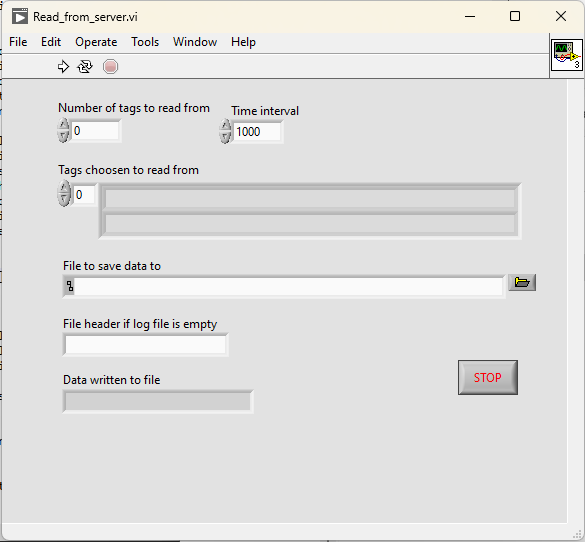
\includegraphics[width=8cm, height=8cm]{Labview OPC DA/builds/Read from server/Read_Screenshot.png}
\caption{A screenshot of the LabView OPC DA server reader application. the user can decide different inputs, and recieve information back from the server.}
\label{im:L_DA_R}
				\end{figure}
In figure \ref{im:L_DA_R} it is shown that the reading application consists of a simple GUI where the user can choose the number of tags to be read and time interval of reading. The file to be written to can also be chosen, and if that file is empty a possible header for the file can be given. \\
				\begin{figure}
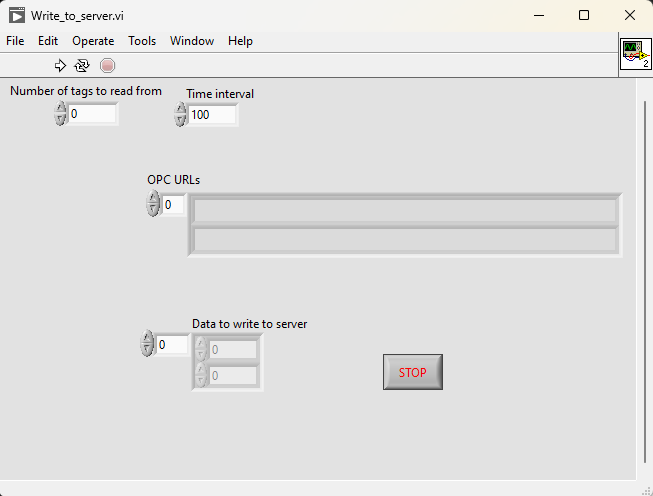
\includegraphics[width=8cm, height=8cm]{Labview OPC DA/builds/Write to server/Write_Screenshot.png}
\caption{A screenshot of the LabView OPC DA server writer application. It is show that the design is similar to the reader, with different input being given and the Server URL being displayed.}
\label{im:L_DA_W}
				\end{figure}
In figure \ref{im:L_DA_W} it is possible to see that the writing application is similar to the reading application, but with fewer elements. The number of tags, time interval and the display for OPC URL are the same, just with different names. However there is an input element where the user can write what data they want to write to the server, which replaces the file selection and output element of the reader. \\
				\begin{figure}[H]
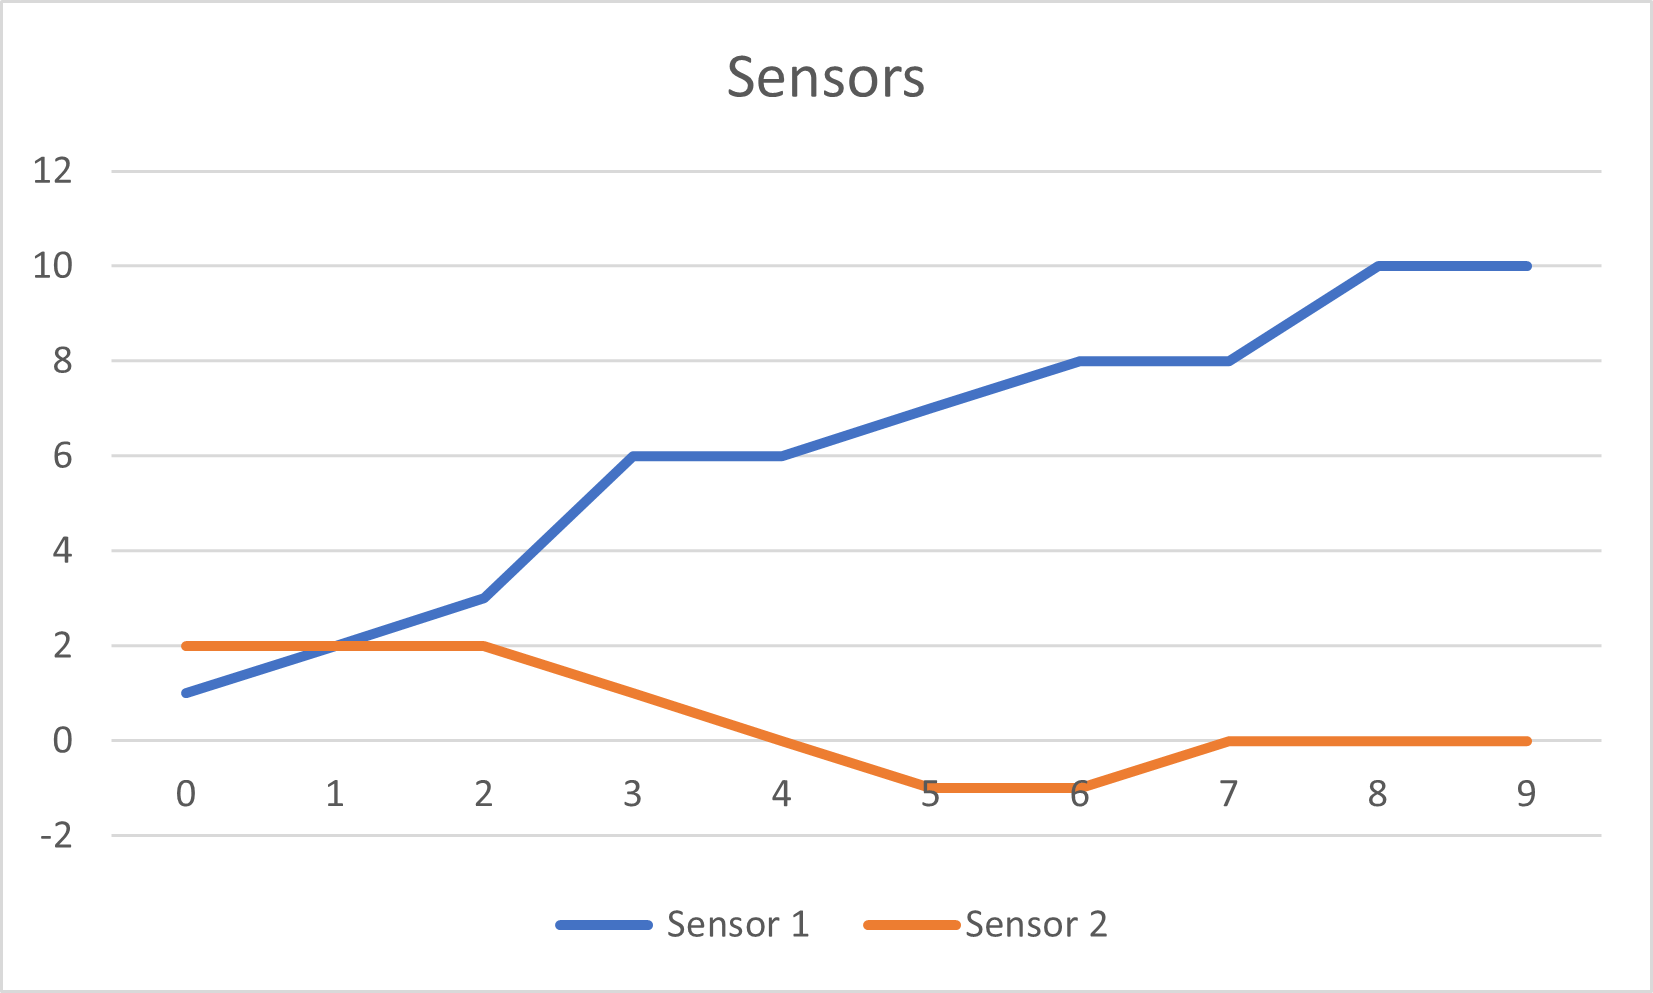
\includegraphics[width=12.8cm, height=8cm]{Labview OPC DA/Sensors graph.png}
\caption{A plot of the data produced from running the application with two tags.}
\label{im:L_DA_D}
				\end{figure}
The resulting data read from a single running of the program, with two tags,  and plotted using Microsoft Excel can be seen in figure \ref{im:L_DA_D}.

			\subsubsection{LabView UA Application}
As for the LabView UA application, this also uses the Q1 2024 version of LabView, but with the added package LabView OPC UA Toolkit. This application includes three parts. The clients, which read and write from the server, each connect to the sever using a string input from the user and the Connect.vi. Then they enter a while loop and interact with the server using either a Multiple Read- or Multiple Write.vi continuously with fixed time intervals. Finally, they disconnect from the server and handle any problems.
				\begin{figure}
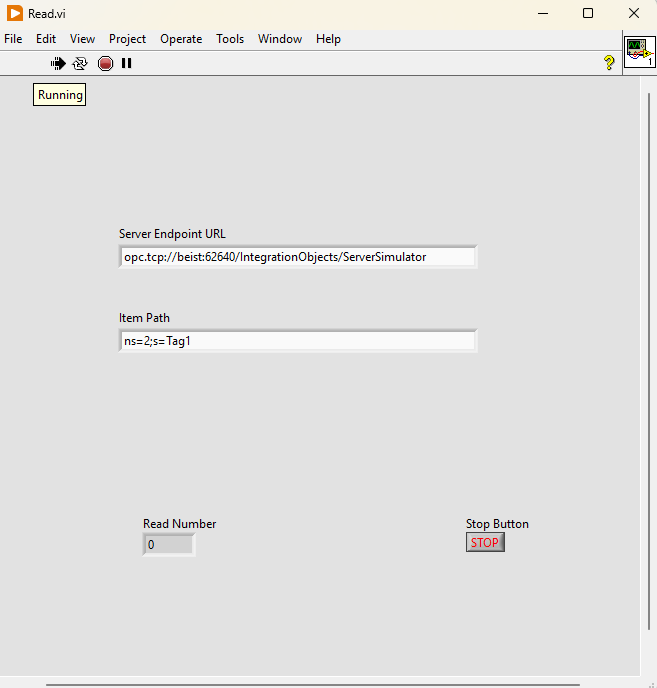
\includegraphics[width=8cm, height=8cm]{Labview OPC UA/Client/Read_Screenshot.png}
\caption{A screenshot of the LabView OPC UA server reader application. The design is similar to the DA reader, but it only displays the data read and doesn't allow for multiple tags to be read.}
\label{im:L_UA_R}
				\end{figure}
				\begin{figure}
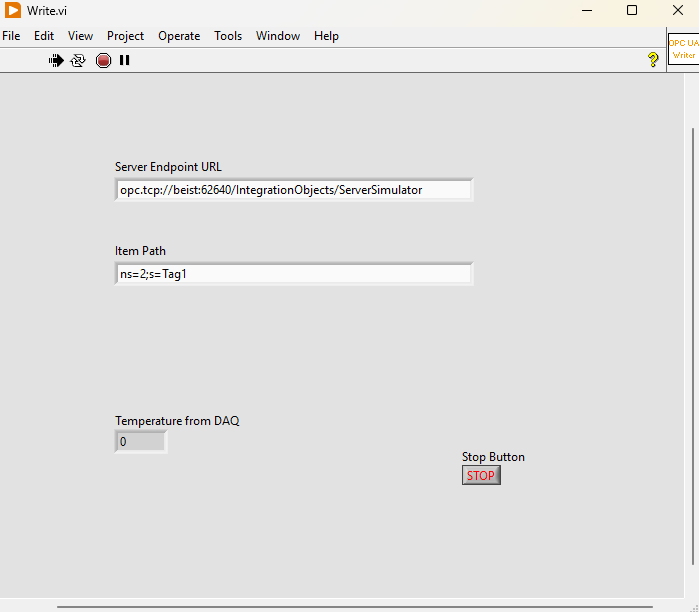
\includegraphics[width=8cm, height=8cm]{Labview OPC UA/Client/Write_Screenshot.png}
\caption{A screenshot of the LabView OPC UA server writer application. Almost identical to the reader except the indicator for data is what is being written to the server and not what has been read.}
\label{im:L_UA_W}
				\end{figure}
The reader displays the value of a single tag read from the server as seen in figure \ref{im:L_UA_R}, while the writer gets a random value generated, to simulate a sensor input, and displays this value as seen in figure \ref{im:L_UA_W}, while writing it to a single tag. 
				\begin{figure}
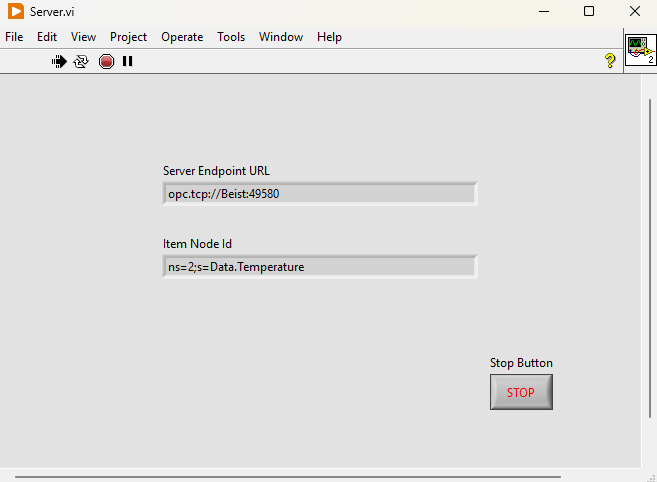
\includegraphics[width=8cm, height=8cm]{Labview OPC UA/Server/Server_Screenshot.png}
\caption{A screenshot of the LabView OPC UA server application. Almost identical to the reader and writer, except it lacks an indicator for data.}
\label{im:L_UA_S}
				\end{figure}
The final part of the application is a server, set up with a single tag, which is capable of being read from and written to. The server, seen in figure \ref{im:L_UA_S} starts by opening a server using the Create.vi. Then it creates a folder with the name Data and an item with the name Temperature, type double and both read and write access. Finally, it starts the server with Start.vi and enters a while loop and when exiting the while loop it stops and closes the server.
			
			\subsubsection{C\# Application}
The C\# application is a single program, as seen in figure \ref{im:C}, which can both read and write itself. It was built using Visual Studio and the NuGet Package Opc UaFx Client version 2.41.1.
				\begin{figure}
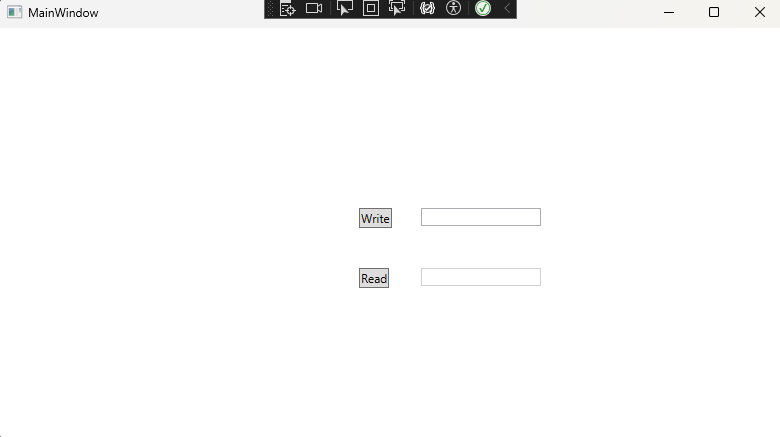
\includegraphics[width=12.8cm, height=8cm]{Csharp OPC UA Client/Program_Screenshot.png}
\caption{A screenshot of the C\# OPC UA application built from debugging in Visual Studio. There is a window for input to what should be written to the server and two buttons. One button writes the user input to the server and one reads from server.}
\label{im:C}
				\end{figure}
The program connects to the server each time it is prompted to do so by the user, either to read from or write to the server. The user can specify a number to be written to the server by filling in the input box to the right of the write button.

			\subsubsection{Python Application}
The finale application was created using the programming language Python, and the package Opcua.
				\begin{figure}[h]
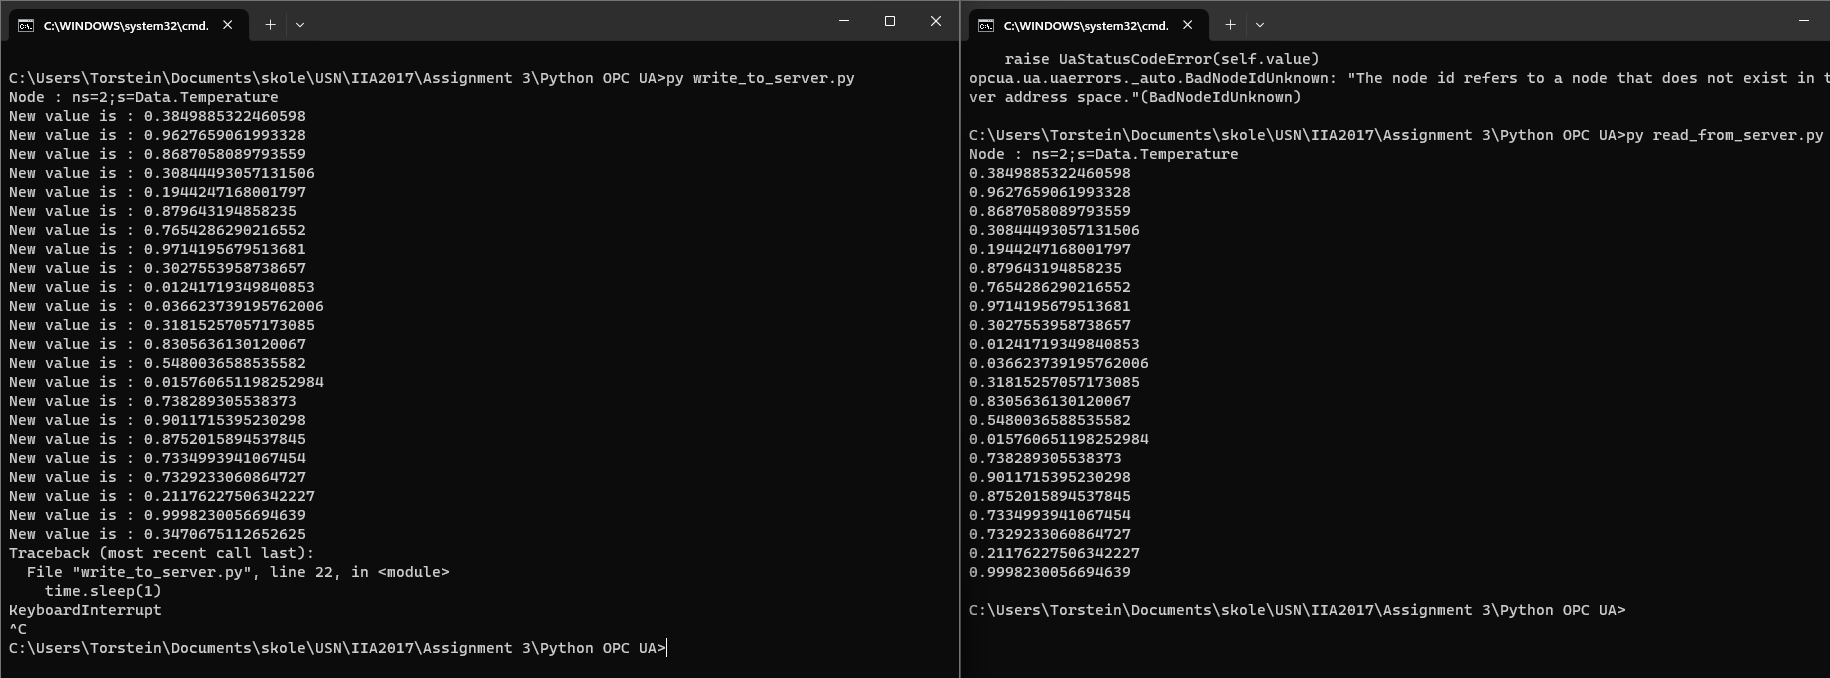
\includegraphics[width=12.8cm, height=7cm]{Python OPC UA/Program_Screenshot.png}
\caption{A screenshot of the Python OPC UA reader and writer applications ran using CMD. These programs reads and writes a tags value and prints the value to the terminal.}
\label{im:P}
				\end{figure}
The application consists of a reading and a writing program, each which connects to the server using Opcua and then enter a while loop where they perform their task. At some point, the user interrupts the code with a keyboard interrupt, and the programs perform any last tasks, disconnects from the server and ends. The reader, as seen in figure \ref{im:P} reads the value of a tag from the server and prints it to the terminal as well as a .csv file. The writer, as seen in figure \ref{im:P}, gets a random number from the random package and writes this to the server.

		\subsection{Communication Test}
Each application where tested by running the program up against their partner. Meaning that the reader programs and writer programs from each application where tested together. They where also tested using different servers, and the results of the tests can be seen in table \ref{tb:res}
			\begin{table}

\noindent 		\begin{tabularx}{\linewidth}{@{}|X|X|X|}
\hline
Application    & Server                                         & Result \\
\hline
LabView OPC DA & Matrikon OPC Simulation Server \cite{Matrikon}	& Worked \\
LabView OPC UA & Selfmade LabView OPC UA Server					& Worked \\
LabView OPC DA & OPC UA Server Simulator \cite{IO}	            & Worked \\
LabView OPC DA & Selfmade LabView OPC UA Server 				& Worked \\
\hline
				\end{tabularx}
\caption{The result from testing each of the applications. All the applications work.}
\label{tb:res}
			\end{table}
The table shows that all the applications work at that the server made in LabView also works. There are two server simulators used as well, one from Matrikon and one from Integration Objects.

		\subsection{Network Communication Test}
The network communication test was performed only on the python application, and a screenshot of the resulting datafiles and a plot of the data produced are shown in figure \ref{im:N_S} and \ref{im:N_D} respectively. \\
			\begin{figure}[H]
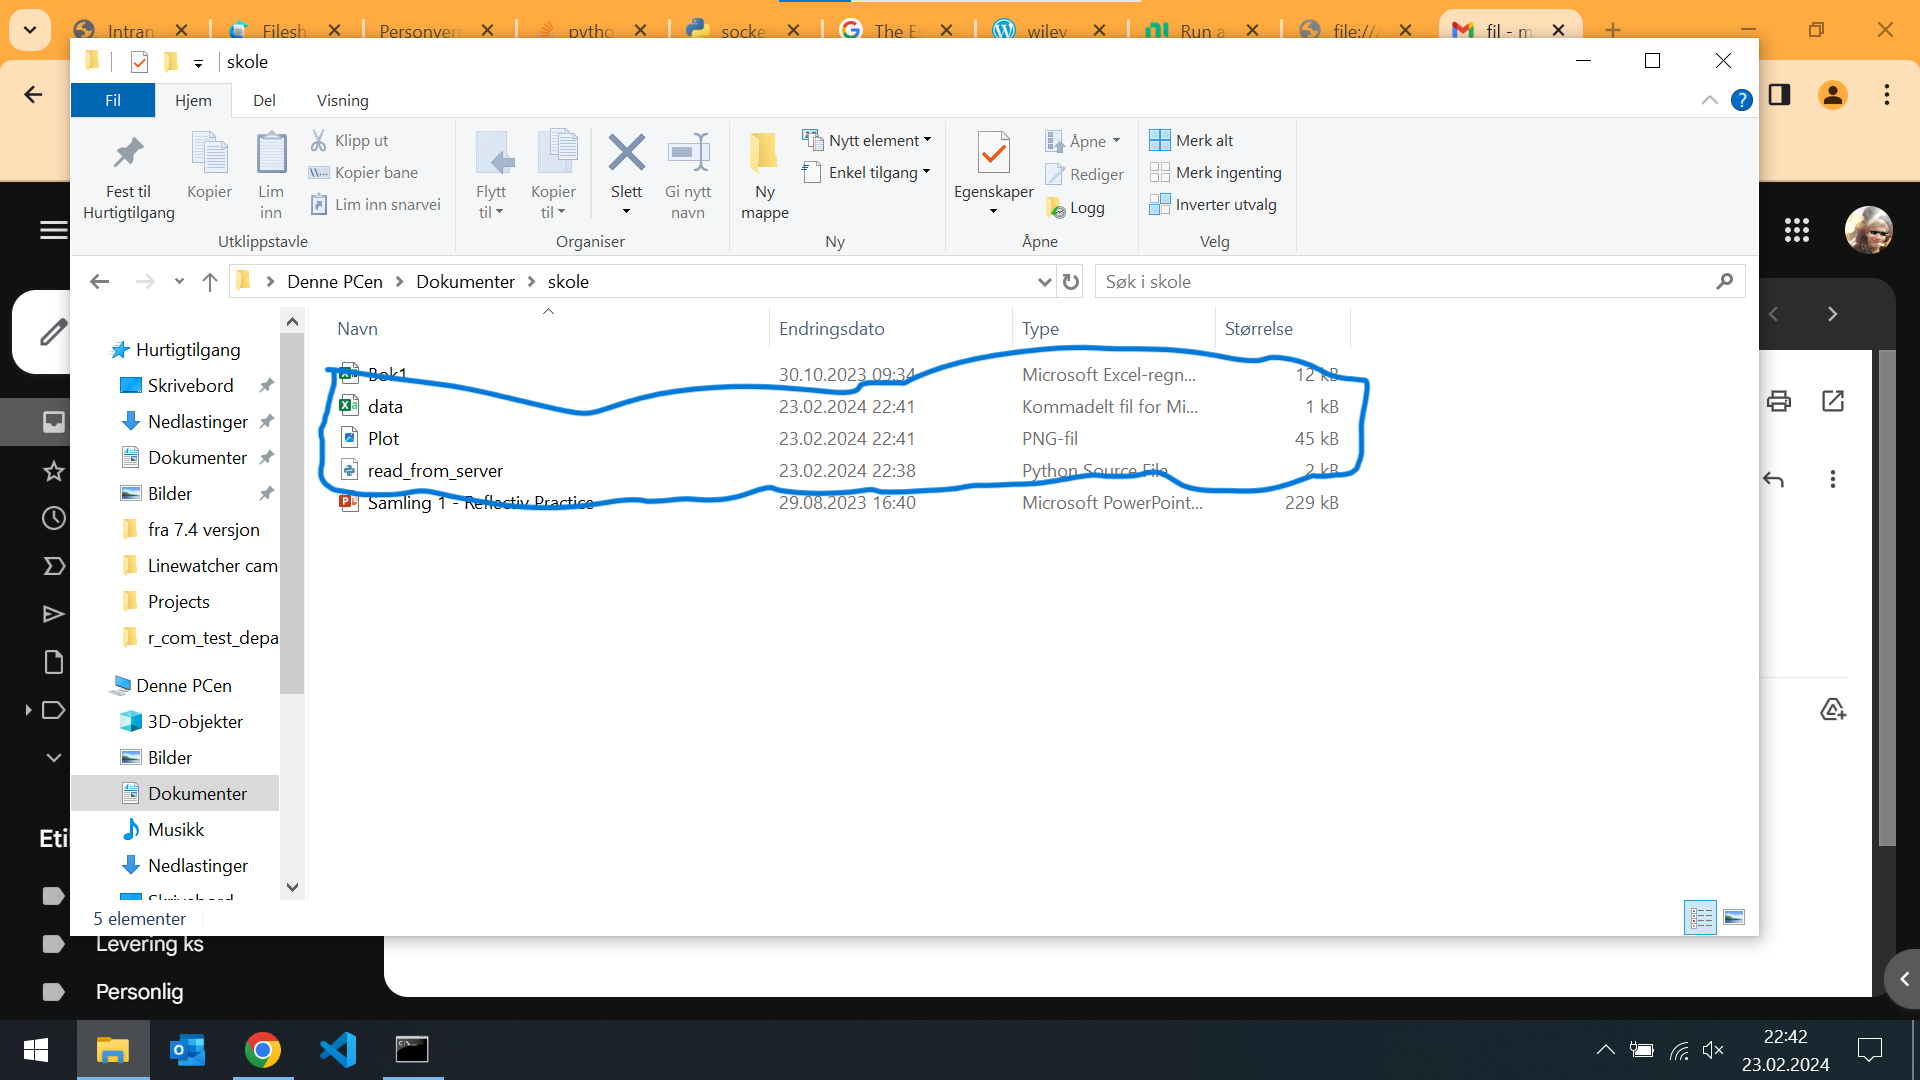
\includegraphics[width=12.8cm, height=8cm]{Skjermbilde 2024-02-23 224305.png}
\caption{A screenshot of the C\# OPC UA application built from debugging in Visual Studio. There is a window for input to what should be written to the server and two buttons. One button writes the user input to the server and one reads from server.}
\label{im:N_S}
			\end{figure}
			\begin{figure}[H]
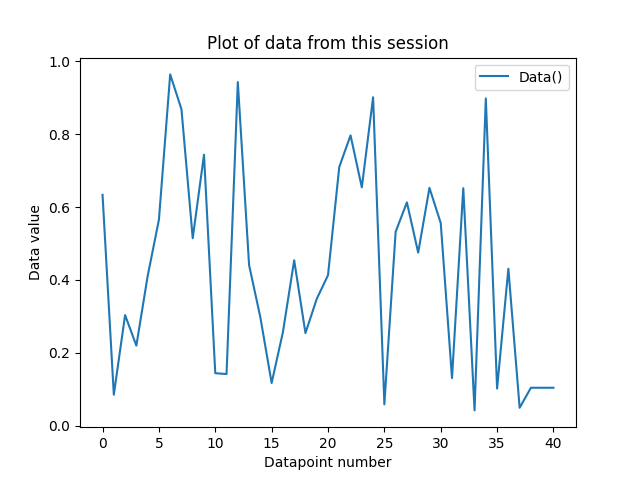
\includegraphics[width=12.8cm, height=8cm]{Plot.png}
\caption{A screenshot of the C\# OPC UA application built from debugging in Visual Studio. There is a window for input to what should be written to the server and two buttons. One button writes the user input to the server and one reads from server.}
\label{im:N_D}
			\end{figure}
The figures show that the reader was run from a different pc and that two files where created as expected. They also show that the data read was not empty or a single value, but changing throughout the running.

	\section{Discussion}
Each of the applications work and can perform the task of writing data to an OPC server and reading it from the server. Some of the applications can save the data to files and one of them can also plot the data as well. The applications answer the task outlined in the competition, but do little more. The combination of all the different applications into a single one with the capabilities off reading, writing saving to file and plotting, as well as prompting the user to choose the server and tag, and how many tags to choose would have been optimal. \\
The applications should also be tested more thoroughly, not just up against their own partners, but also each others. They should also have been tested up against different servers. If more time had been available this would have been the next step. Furthermore, as there was only one other computer available during the production of these applications, and this computer did not have administrative rights, the only application which could be tested over a network was the one which that computer already had the software for. This was the Python application, and with more funds It would have been possible to rent another device and test the other applications as well. This was also the reason why Python was chosen in stead of MATLAB which the contest listed as preferred, but since Python was the only software possible to test over a network, and the contest said other software could be used, Python was chosen. \\
Finally, a test where actual sensors and not just simulated sensors where used would have been beneficial, so as to make sure this would not produce complications, but as with the network test, there where no funds for such a test and this was cut from the scope. \\
If this article should recommend the use of one of these applications, it would be the LabView OPC DA application, as it has the most features and could be used with little extra development.

	\section{Conclusion}
The contest, posted by Not At All Made Up Industrial Production Company, has been answered, and four OPC server interaction applications have been produced. The are all capable of reading from and writing data to an OPC server, but lack some testing and should possibly have been combined into a single application with the abilities all of them. However, the best one of the four is most likely the LabView OPC DA application as it has the most features.

\printbibliography
	
	\section{Appendix A}
Here you can find the documentation for the applications: \\
		\begin{figure}[H]
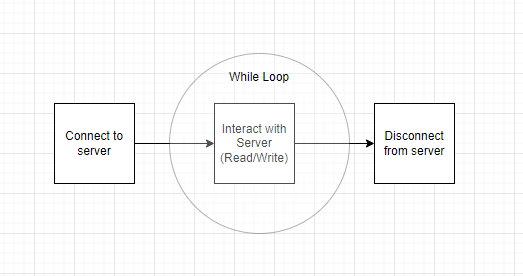
\includegraphics[width=12.8cm, height=8cm]{Flowchart.png}
\caption{Flowchart depicting the general flow of all the applications. The applications all connect to a server, enter a while loop where they interact with the server, and finally, exit the loop and disconnect from the server.}
\label{im:flow}
		\end{figure}
Figure \ref{im:flow} shows the general build up of all the applications. All applications are build up in the same way, connection to the server, interacting with it inside a while loop, and finally disconnecting from the server when exiting the while loop.

	\section{Appendix B}
All code can be found on the projects GitHub repository \cite{github}. As listing the code in this rapport would be long and hard thing to read, this way has been chosen.

\end{document}